\documentclass[twoside]{book}

% Packages required by doxygen
\usepackage{fixltx2e}
\usepackage{calc}
\usepackage{doxygen}
\usepackage[export]{adjustbox} % also loads graphicx
\usepackage{graphicx}
\usepackage[utf8]{inputenc}
\usepackage{makeidx}
\usepackage{multicol}
\usepackage{multirow}
\PassOptionsToPackage{warn}{textcomp}
\usepackage{textcomp}
\usepackage[nointegrals]{wasysym}
\usepackage[table]{xcolor}

% Font selection
\usepackage[T1]{fontenc}
\usepackage[scaled=.90]{helvet}
\usepackage{courier}
\usepackage{amssymb}
\usepackage{sectsty}
\renewcommand{\familydefault}{\sfdefault}
\allsectionsfont{%
  \fontseries{bc}\selectfont%
  \color{darkgray}%
}
\renewcommand{\DoxyLabelFont}{%
  \fontseries{bc}\selectfont%
  \color{darkgray}%
}
\newcommand{\+}{\discretionary{\mbox{\scriptsize$\hookleftarrow$}}{}{}}

% Page & text layout
\usepackage{geometry}
\geometry{%
  a4paper,%
  top=2.5cm,%
  bottom=2.5cm,%
  left=2.5cm,%
  right=2.5cm%
}
\tolerance=750
\hfuzz=15pt
\hbadness=750
\setlength{\emergencystretch}{15pt}
\setlength{\parindent}{0cm}
\setlength{\parskip}{3ex plus 2ex minus 2ex}
\makeatletter
\renewcommand{\paragraph}{%
  \@startsection{paragraph}{4}{0ex}{-1.0ex}{1.0ex}{%
    \normalfont\normalsize\bfseries\SS@parafont%
  }%
}
\renewcommand{\subparagraph}{%
  \@startsection{subparagraph}{5}{0ex}{-1.0ex}{1.0ex}{%
    \normalfont\normalsize\bfseries\SS@subparafont%
  }%
}
\makeatother

% Headers & footers
\usepackage{fancyhdr}
\pagestyle{fancyplain}
\fancyhead[LE]{\fancyplain{}{\bfseries\thepage}}
\fancyhead[CE]{\fancyplain{}{}}
\fancyhead[RE]{\fancyplain{}{\bfseries\leftmark}}
\fancyhead[LO]{\fancyplain{}{\bfseries\rightmark}}
\fancyhead[CO]{\fancyplain{}{}}
\fancyhead[RO]{\fancyplain{}{\bfseries\thepage}}
\fancyfoot[LE]{\fancyplain{}{}}
\fancyfoot[CE]{\fancyplain{}{}}
\fancyfoot[RE]{\fancyplain{}{\bfseries\scriptsize Generated by Doxygen }}
\fancyfoot[LO]{\fancyplain{}{\bfseries\scriptsize Generated by Doxygen }}
\fancyfoot[CO]{\fancyplain{}{}}
\fancyfoot[RO]{\fancyplain{}{}}
\renewcommand{\footrulewidth}{0.4pt}
\renewcommand{\chaptermark}[1]{%
  \markboth{#1}{}%
}
\renewcommand{\sectionmark}[1]{%
  \markright{\thesection\ #1}%
}

% Indices & bibliography
\usepackage{natbib}
\usepackage[titles]{tocloft}
\setcounter{tocdepth}{3}
\setcounter{secnumdepth}{5}
\makeindex

% Hyperlinks (required, but should be loaded last)
\usepackage{ifpdf}
\ifpdf
  \usepackage[pdftex,pagebackref=true]{hyperref}
\else
  \usepackage[ps2pdf,pagebackref=true]{hyperref}
\fi
\hypersetup{%
  colorlinks=true,%
  linkcolor=blue,%
  citecolor=blue,%
  unicode%
}

% Custom commands
\newcommand{\clearemptydoublepage}{%
  \newpage{\pagestyle{empty}\cleardoublepage}%
}

\usepackage{caption}
\captionsetup{labelsep=space,justification=centering,font={bf},singlelinecheck=off,skip=4pt,position=top}

%===== C O N T E N T S =====

\begin{document}

% Titlepage & ToC
\hypersetup{pageanchor=false,
             bookmarksnumbered=true,
             pdfencoding=unicode
            }
\pagenumbering{alph}
\begin{titlepage}
\vspace*{7cm}
\begin{center}%
{\Large \textquotesingle{}H\+C-\/\+S\+R04\+\_\+\+\_\+driver\+\_\+\+\_\+for\+\_\+\+\_\+\+R\+I\+O\+T-\/\+OS\textquotesingle{} }\\
\vspace*{1cm}
{\large Generated by Doxygen 1.8.13}\\
\end{center}
\end{titlepage}
\clearemptydoublepage
\pagenumbering{roman}
\tableofcontents
\clearemptydoublepage
\pagenumbering{arabic}
\hypersetup{pageanchor=true}

%--- Begin generated contents ---
\chapter{Module Index}
\section{Modules}
Here is a list of all modules\+:\begin{DoxyCompactList}
\item \contentsline{section}{H\+C-\/\+S\+R04}{\pageref{group__drivers__hcsr04}}{}
\end{DoxyCompactList}

\chapter{Class Index}
\section{Class List}
Here are the classes, structs, unions and interfaces with brief descriptions\+:\begin{DoxyCompactList}
\item\contentsline{section}{\hyperlink{structhcsr04__params__t}{hcsr04\+\_\+params\+\_\+t} \\*Device initialization parameters for hcsr04 sensor }{\pageref{structhcsr04__params__t}}{}
\item\contentsline{section}{\hyperlink{structhcsr04__t}{hcsr04\+\_\+t} \\*Device descriptor of a H\+C-\/\+S\+R04 sensor }{\pageref{structhcsr04__t}}{}
\end{DoxyCompactList}

\chapter{File Index}
\section{File List}
Here is a list of all documented files with brief descriptions\+:\begin{DoxyCompactList}
\item\contentsline{section}{/home/evripidis/\+Documents/diploma/\+R\+I\+O\+T/drivers/hcsr04/\hyperlink{hcsr04_8c}{hcsr04.\+c} \\*Device driver implementation for the H\+C-\/\+S\+R04 }{\pageref{hcsr04_8c}}{}
\item\contentsline{section}{/home/evripidis/\+Documents/diploma/\+R\+I\+O\+T/drivers/hcsr04/include/\hyperlink{hcsr04__constants_8h}{hcsr04\+\_\+constants.\+h} \\*Internal addresses, registers and constants }{\pageref{hcsr04__constants_8h}}{}
\item\contentsline{section}{/home/evripidis/\+Documents/diploma/\+R\+I\+O\+T/drivers/hcsr04/include/\hyperlink{hcsr04__params_8h}{hcsr04\+\_\+params.\+h} \\*Default configuration }{\pageref{hcsr04__params_8h}}{}
\item\contentsline{section}{/home/evripidis/\+Documents/diploma/\+R\+I\+O\+T/drivers/include/\hyperlink{hcsr04_8h}{hcsr04.\+h} }{\pageref{hcsr04_8h}}{}
\end{DoxyCompactList}

\chapter{Module Documentation}
\hypertarget{group__drivers__hcsr04}{}\section{H\+C-\/\+S\+R04}
\label{group__drivers__hcsr04}\index{H\+C-\/\+S\+R04@{H\+C-\/\+S\+R04}}


This is a sensor which uses ultrasonic waves in order to measure the distance.  


\subsection*{Files}
\begin{DoxyCompactItemize}
\item 
file \hyperlink{hcsr04_8c}{hcsr04.\+c}
\begin{DoxyCompactList}\small\item\em Device driver implementation for the H\+C-\/\+S\+R04. \end{DoxyCompactList}\item 
file \hyperlink{hcsr04__constants_8h}{hcsr04\+\_\+constants.\+h}
\begin{DoxyCompactList}\small\item\em Internal addresses, registers and constants. \end{DoxyCompactList}\item 
file \hyperlink{hcsr04__params_8h}{hcsr04\+\_\+params.\+h}
\begin{DoxyCompactList}\small\item\em Default configuration. \end{DoxyCompactList}\item 
file \hyperlink{hcsr04_8h}{hcsr04.\+h}
\end{DoxyCompactItemize}
\subsection*{Classes}
\begin{DoxyCompactItemize}
\item 
struct \hyperlink{structhcsr04__params__t}{hcsr04\+\_\+params\+\_\+t}
\begin{DoxyCompactList}\small\item\em Device initialization parameters for hcsr04 sensor. \end{DoxyCompactList}\item 
struct \hyperlink{structhcsr04__t}{hcsr04\+\_\+t}
\begin{DoxyCompactList}\small\item\em Device descriptor of a H\+C-\/\+S\+R04 sensor. \end{DoxyCompactList}\end{DoxyCompactItemize}
\subsection*{Functions}
\begin{DoxyCompactItemize}
\item 
int \hyperlink{group__drivers__hcsr04_gabcca3ead68bf012ae42e185e070cb764}{hcsr04\+\_\+init} (\hyperlink{structhcsr04__t}{hcsr04\+\_\+t} $\ast$dev, const \hyperlink{structhcsr04__params__t}{hcsr04\+\_\+params\+\_\+t} $\ast$params)
\begin{DoxyCompactList}\small\item\em Initialize an H\+C-\/\+S\+R04 sensor. \end{DoxyCompactList}\item 
void \hyperlink{group__drivers__hcsr04_gabbfe6e650342e8cc67cf9c9e81b29335}{hcsr04\+\_\+trigger} (\hyperlink{structhcsr04__t}{hcsr04\+\_\+t} $\ast$dev)
\begin{DoxyCompactList}\small\item\em Starts a measurement by triggering the H\+C-\/\+S\+R04 device. \end{DoxyCompactList}\item 
uint16\+\_\+t \hyperlink{group__drivers__hcsr04_ga449b9d4dc30d3d87d9ee4d8936fb592d}{hcsr04\+\_\+read} (\hyperlink{structhcsr04__t}{hcsr04\+\_\+t} $\ast$dev)
\begin{DoxyCompactList}\small\item\em Gets the last measurement reading. \end{DoxyCompactList}\item 
uint16\+\_\+t \hyperlink{group__drivers__hcsr04_ga3b2547facab2613e3113c2fd5d2bd6a8}{hcsr04\+\_\+temp\+\_\+to\+\_\+sound\+\_\+speed} (uint16\+\_\+t temp)
\begin{DoxyCompactList}\small\item\em Function that calculates the speed of sound. \end{DoxyCompactList}\item 
void \hyperlink{group__drivers__hcsr04_gad5a6694b723bb25fc48e7a8750b8a77a}{hcsr04\+\_\+set\+\_\+temp} (\hyperlink{structhcsr04__t}{hcsr04\+\_\+t} $\ast$dev, uint16\+\_\+t new\+\_\+temp)
\begin{DoxyCompactList}\small\item\em Function that sets the temperature. \end{DoxyCompactList}\item 
uint16\+\_\+t \hyperlink{group__drivers__hcsr04_gabef54fa09a72a7aa863aaa03b662125b}{hcsr04\+\_\+get\+\_\+distance} (\hyperlink{structhcsr04__t}{hcsr04\+\_\+t} $\ast$dev)
\begin{DoxyCompactList}\small\item\em Function that measures the current distance. \end{DoxyCompactList}\end{DoxyCompactItemize}


\subsection{Detailed Description}
This is a sensor which uses ultrasonic waves in order to measure the distance. 



\subsection{Function Documentation}
\mbox{\Hypertarget{group__drivers__hcsr04_gabef54fa09a72a7aa863aaa03b662125b}\label{group__drivers__hcsr04_gabef54fa09a72a7aa863aaa03b662125b}} 
\index{H\+C-\/\+S\+R04@{H\+C-\/\+S\+R04}!hcsr04\+\_\+get\+\_\+distance@{hcsr04\+\_\+get\+\_\+distance}}
\index{hcsr04\+\_\+get\+\_\+distance@{hcsr04\+\_\+get\+\_\+distance}!H\+C-\/\+S\+R04@{H\+C-\/\+S\+R04}}
\subsubsection{\texorpdfstring{hcsr04\+\_\+get\+\_\+distance()}{hcsr04\_get\_distance()}}
{\footnotesize\ttfamily uint16\+\_\+t hcsr04\+\_\+get\+\_\+distance (\begin{DoxyParamCaption}\item[{\hyperlink{structhcsr04__t}{hcsr04\+\_\+t} $\ast$}]{dev }\end{DoxyParamCaption})}



Function that measures the current distance. 


\begin{DoxyParams}[1]{Parameters}
\mbox{\tt in,out}  & {\em arg} & Device descriptor of the driver\\
\hline
\end{DoxyParams}
Internally it calls the \hyperlink{group__drivers__hcsr04_gabbfe6e650342e8cc67cf9c9e81b29335}{hcsr04\+\_\+trigger} \& \hyperlink{group__drivers__hcsr04_ga449b9d4dc30d3d87d9ee4d8936fb592d}{hcsr04\+\_\+read} with the ideal minimum time interval based on the datasheet \mbox{\Hypertarget{group__drivers__hcsr04_gabcca3ead68bf012ae42e185e070cb764}\label{group__drivers__hcsr04_gabcca3ead68bf012ae42e185e070cb764}} 
\index{H\+C-\/\+S\+R04@{H\+C-\/\+S\+R04}!hcsr04\+\_\+init@{hcsr04\+\_\+init}}
\index{hcsr04\+\_\+init@{hcsr04\+\_\+init}!H\+C-\/\+S\+R04@{H\+C-\/\+S\+R04}}
\subsubsection{\texorpdfstring{hcsr04\+\_\+init()}{hcsr04\_init()}}
{\footnotesize\ttfamily int hcsr04\+\_\+init (\begin{DoxyParamCaption}\item[{\hyperlink{structhcsr04__t}{hcsr04\+\_\+t} $\ast$}]{dev,  }\item[{const \hyperlink{structhcsr04__params__t}{hcsr04\+\_\+params\+\_\+t} $\ast$}]{params }\end{DoxyParamCaption})}



Initialize an H\+C-\/\+S\+R04 sensor. 


\begin{DoxyParams}[1]{Parameters}
\mbox{\tt in,out}  & {\em dev} & Device descriptor of the driver \\
\hline
\mbox{\tt in}  & {\em params} & Initialization parameters\\
\hline
\end{DoxyParams}
\begin{DoxyReturn}{Returns}
E\+IO of invalid parameters 

E\+C\+ON if connection issue is detected 

0 on success
\end{DoxyReturn}
After called it checks the parameters, calculates the sound speed based on the default temperature, initializes the hardware and performs a check reading to see if the sensor\textquotesingle{}s echo pin works \mbox{\Hypertarget{group__drivers__hcsr04_ga449b9d4dc30d3d87d9ee4d8936fb592d}\label{group__drivers__hcsr04_ga449b9d4dc30d3d87d9ee4d8936fb592d}} 
\index{H\+C-\/\+S\+R04@{H\+C-\/\+S\+R04}!hcsr04\+\_\+read@{hcsr04\+\_\+read}}
\index{hcsr04\+\_\+read@{hcsr04\+\_\+read}!H\+C-\/\+S\+R04@{H\+C-\/\+S\+R04}}
\subsubsection{\texorpdfstring{hcsr04\+\_\+read()}{hcsr04\_read()}}
{\footnotesize\ttfamily uint16\+\_\+t hcsr04\+\_\+read (\begin{DoxyParamCaption}\item[{\hyperlink{structhcsr04__t}{hcsr04\+\_\+t} $\ast$}]{dev }\end{DoxyParamCaption})}



Gets the last measurement reading. 


\begin{DoxyParams}[1]{Parameters}
\mbox{\tt in,out}  & {\em dev} & Device descriptor of the driver\\
\hline
\end{DoxyParams}
This function returns the distance in milli meters

\begin{DoxyWarning}{Warning}
Before read a value \hyperlink{group__drivers__hcsr04_gabbfe6e650342e8cc67cf9c9e81b29335}{hcsr04\+\_\+trigger} has to be called
\end{DoxyWarning}
\begin{DoxyNote}{Note}
This function will retrieve the calculated distance after the last trigger 
\end{DoxyNote}
\mbox{\Hypertarget{group__drivers__hcsr04_gad5a6694b723bb25fc48e7a8750b8a77a}\label{group__drivers__hcsr04_gad5a6694b723bb25fc48e7a8750b8a77a}} 
\index{H\+C-\/\+S\+R04@{H\+C-\/\+S\+R04}!hcsr04\+\_\+set\+\_\+temp@{hcsr04\+\_\+set\+\_\+temp}}
\index{hcsr04\+\_\+set\+\_\+temp@{hcsr04\+\_\+set\+\_\+temp}!H\+C-\/\+S\+R04@{H\+C-\/\+S\+R04}}
\subsubsection{\texorpdfstring{hcsr04\+\_\+set\+\_\+temp()}{hcsr04\_set\_temp()}}
{\footnotesize\ttfamily void hcsr04\+\_\+set\+\_\+temp (\begin{DoxyParamCaption}\item[{\hyperlink{structhcsr04__t}{hcsr04\+\_\+t} $\ast$}]{dev,  }\item[{uint16\+\_\+t}]{new\+\_\+temp }\end{DoxyParamCaption})}



Function that sets the temperature. 


\begin{DoxyParams}[1]{Parameters}
\mbox{\tt in,out}  & {\em arg} & Device descriptor of the driver \\
\hline
\mbox{\tt in,out}  & {\em new\+\_\+temp} & New temperature in mili Celsious\\
\hline
\end{DoxyParams}
Internally it calls \hyperlink{group__drivers__hcsr04_ga3b2547facab2613e3113c2fd5d2bd6a8}{hcsr04\+\_\+temp\+\_\+to\+\_\+sound\+\_\+speed} to calculate the speed of sound so the distance calculation is more accurate \mbox{\Hypertarget{group__drivers__hcsr04_ga3b2547facab2613e3113c2fd5d2bd6a8}\label{group__drivers__hcsr04_ga3b2547facab2613e3113c2fd5d2bd6a8}} 
\index{H\+C-\/\+S\+R04@{H\+C-\/\+S\+R04}!hcsr04\+\_\+temp\+\_\+to\+\_\+sound\+\_\+speed@{hcsr04\+\_\+temp\+\_\+to\+\_\+sound\+\_\+speed}}
\index{hcsr04\+\_\+temp\+\_\+to\+\_\+sound\+\_\+speed@{hcsr04\+\_\+temp\+\_\+to\+\_\+sound\+\_\+speed}!H\+C-\/\+S\+R04@{H\+C-\/\+S\+R04}}
\subsubsection{\texorpdfstring{hcsr04\+\_\+temp\+\_\+to\+\_\+sound\+\_\+speed()}{hcsr04\_temp\_to\_sound\_speed()}}
{\footnotesize\ttfamily uint16\+\_\+t hcsr04\+\_\+temp\+\_\+to\+\_\+sound\+\_\+speed (\begin{DoxyParamCaption}\item[{uint16\+\_\+t}]{temp }\end{DoxyParamCaption})}



Function that calculates the speed of sound. 


\begin{DoxyParams}[1]{Parameters}
\mbox{\tt in,out}  & {\em temp} & Temperature in mili Celsious\\
\hline
\end{DoxyParams}
It uses the following formula\+: v = s $\ast$ sqrt(1 + T/\+To) Where\+:
\begin{DoxyItemize}
\item s is the speed of sound at 0 Celsious or 273 Kelvin
\item T is the given air temperature
\item To is the reference temperature 273 Kelvin
\end{DoxyItemize}

\begin{DoxyWarning}{Warning}
Temperature must be given in milli Celsious 
\end{DoxyWarning}
\mbox{\Hypertarget{group__drivers__hcsr04_gabbfe6e650342e8cc67cf9c9e81b29335}\label{group__drivers__hcsr04_gabbfe6e650342e8cc67cf9c9e81b29335}} 
\index{H\+C-\/\+S\+R04@{H\+C-\/\+S\+R04}!hcsr04\+\_\+trigger@{hcsr04\+\_\+trigger}}
\index{hcsr04\+\_\+trigger@{hcsr04\+\_\+trigger}!H\+C-\/\+S\+R04@{H\+C-\/\+S\+R04}}
\subsubsection{\texorpdfstring{hcsr04\+\_\+trigger()}{hcsr04\_trigger()}}
{\footnotesize\ttfamily void hcsr04\+\_\+trigger (\begin{DoxyParamCaption}\item[{\hyperlink{structhcsr04__t}{hcsr04\+\_\+t} $\ast$}]{dev }\end{DoxyParamCaption})}



Starts a measurement by triggering the H\+C-\/\+S\+R04 device. 


\begin{DoxyParams}[1]{Parameters}
\mbox{\tt in,out}  & {\em dev} & Device descriptor of the driver \\
\hline
\end{DoxyParams}

\chapter{Class Documentation}
\hypertarget{structhcsr04__params__t}{}\section{hcsr04\+\_\+params\+\_\+t Struct Reference}
\label{structhcsr04__params__t}\index{hcsr04\+\_\+params\+\_\+t@{hcsr04\+\_\+params\+\_\+t}}


Device initialization parameters for hcsr04 sensor.  




{\ttfamily \#include $<$hcsr04.\+h$>$}

\subsection*{Public Attributes}
\begin{DoxyCompactItemize}
\item 
\mbox{\Hypertarget{structhcsr04__params__t_a0323d00d2c093e609ee23964326cda6b}\label{structhcsr04__params__t_a0323d00d2c093e609ee23964326cda6b}} 
uint16\+\_\+t {\bfseries temperature}
\item 
\mbox{\Hypertarget{structhcsr04__params__t_a097d9df16ded4968dc873d1dbf73dd47}\label{structhcsr04__params__t_a097d9df16ded4968dc873d1dbf73dd47}} 
gpio\+\_\+t {\bfseries trigger\+\_\+pin}
\item 
\mbox{\Hypertarget{structhcsr04__params__t_a1819d40336759f6fe23b085139e7c094}\label{structhcsr04__params__t_a1819d40336759f6fe23b085139e7c094}} 
gpio\+\_\+t {\bfseries echo\+\_\+pin}
\end{DoxyCompactItemize}


\subsection{Detailed Description}
Device initialization parameters for hcsr04 sensor. 

The documentation for this struct was generated from the following file\+:\begin{DoxyCompactItemize}
\item 
/home/evripidis/\+Documents/diploma/\+R\+I\+O\+T/drivers/include/\hyperlink{hcsr04_8h}{hcsr04.\+h}\end{DoxyCompactItemize}

\hypertarget{structhcsr04__t}{}\section{hcsr04\+\_\+t Struct Reference}
\label{structhcsr04__t}\index{hcsr04\+\_\+t@{hcsr04\+\_\+t}}


Device descriptor of a H\+C-\/\+S\+R04 sensor.  




{\ttfamily \#include $<$hcsr04.\+h$>$}



Collaboration diagram for hcsr04\+\_\+t\+:\nopagebreak
\begin{figure}[H]
\begin{center}
\leavevmode
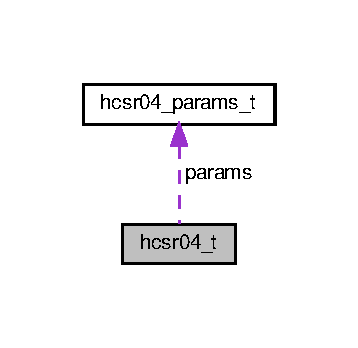
\includegraphics[width=172pt]{structhcsr04__t__coll__graph}
\end{center}
\end{figure}
\subsection*{Public Attributes}
\begin{DoxyCompactItemize}
\item 
\mbox{\Hypertarget{structhcsr04__t_af64d397e8f9cc4ff94941a329499812c}\label{structhcsr04__t_af64d397e8f9cc4ff94941a329499812c}} 
uint16\+\_\+t {\bfseries distance}
\item 
\mbox{\Hypertarget{structhcsr04__t_a644861537571d22723be0ece37ebdbe6}\label{structhcsr04__t_a644861537571d22723be0ece37ebdbe6}} 
uint16\+\_\+t {\bfseries sound\+\_\+speed}
\item 
\mbox{\Hypertarget{structhcsr04__t_aaf349923d0f2ee16de5e9bfc635e3299}\label{structhcsr04__t_aaf349923d0f2ee16de5e9bfc635e3299}} 
uint32\+\_\+t {\bfseries pre\+\_\+timestamp\+\_\+us}
\item 
\mbox{\Hypertarget{structhcsr04__t_a87a029d684f303b03e6139964fd7086a}\label{structhcsr04__t_a87a029d684f303b03e6139964fd7086a}} 
\hyperlink{structhcsr04__params__t}{hcsr04\+\_\+params\+\_\+t} {\bfseries params}
\end{DoxyCompactItemize}


\subsection{Detailed Description}
Device descriptor of a H\+C-\/\+S\+R04 sensor. 

The documentation for this struct was generated from the following file\+:\begin{DoxyCompactItemize}
\item 
/home/evripidis/\+Documents/diploma/\+R\+I\+O\+T/drivers/include/\hyperlink{hcsr04_8h}{hcsr04.\+h}\end{DoxyCompactItemize}

\chapter{File Documentation}
\hypertarget{hcsr04_8c}{}\section{/home/evripidis/\+Documents/diploma/\+R\+I\+O\+T/drivers/hcsr04/hcsr04.c File Reference}
\label{hcsr04_8c}\index{/home/evripidis/\+Documents/diploma/\+R\+I\+O\+T/drivers/hcsr04/hcsr04.\+c@{/home/evripidis/\+Documents/diploma/\+R\+I\+O\+T/drivers/hcsr04/hcsr04.\+c}}


Device driver implementation for the H\+C-\/\+S\+R04.  


{\ttfamily \#include \char`\"{}hcsr04.\+h\char`\"{}}\newline
{\ttfamily \#include \char`\"{}hcsr04\+\_\+constants.\+h\char`\"{}}\newline
{\ttfamily \#include \char`\"{}hcsr04\+\_\+params.\+h\char`\"{}}\newline
{\ttfamily \#include \char`\"{}periph/gpio.\+h\char`\"{}}\newline
{\ttfamily \#include \char`\"{}xtimer.\+h\char`\"{}}\newline
{\ttfamily \#include $<$stdint.\+h$>$}\newline
{\ttfamily \#include $<$errno.\+h$>$}\newline
{\ttfamily \#include $<$math.\+h$>$}\newline
Include dependency graph for hcsr04.\+c\+:\nopagebreak
\begin{figure}[H]
\begin{center}
\leavevmode
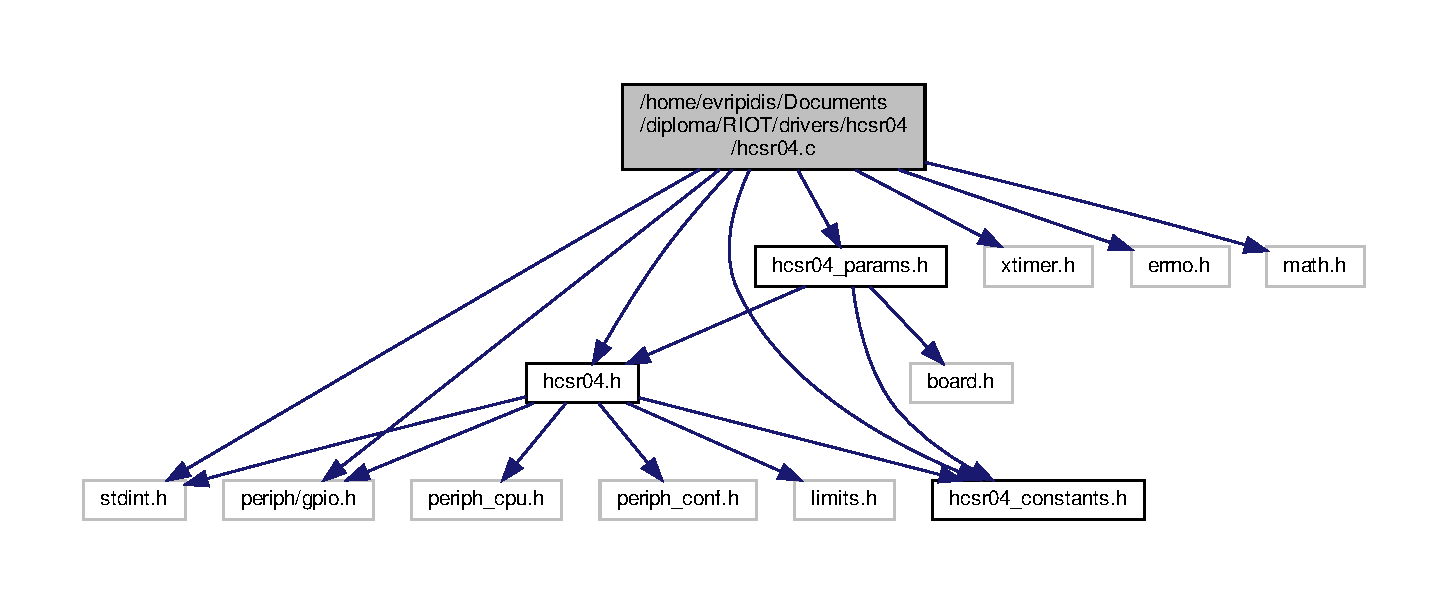
\includegraphics[width=350pt]{hcsr04_8c__incl}
\end{center}
\end{figure}
\subsection*{Functions}
\begin{DoxyCompactItemize}
\item 
\mbox{\Hypertarget{hcsr04_8c_a2834f7c329f56bd4858c056ccb1f7dc6}\label{hcsr04_8c_a2834f7c329f56bd4858c056ccb1f7dc6}} 
void {\bfseries hcsr04\+\_\+int\+\_\+callback} (void $\ast$arg)
\item 
int \hyperlink{group__drivers__hcsr04_gabcca3ead68bf012ae42e185e070cb764}{hcsr04\+\_\+init} (\hyperlink{structhcsr04__t}{hcsr04\+\_\+t} $\ast$dev, const \hyperlink{structhcsr04__params__t}{hcsr04\+\_\+params\+\_\+t} $\ast$params)
\begin{DoxyCompactList}\small\item\em Initialize an H\+C-\/\+S\+R04 sensor. \end{DoxyCompactList}\item 
void \hyperlink{group__drivers__hcsr04_gabbfe6e650342e8cc67cf9c9e81b29335}{hcsr04\+\_\+trigger} (\hyperlink{structhcsr04__t}{hcsr04\+\_\+t} $\ast$dev)
\begin{DoxyCompactList}\small\item\em Starts a measurement by triggering the H\+C-\/\+S\+R04 device. \end{DoxyCompactList}\item 
uint16\+\_\+t \hyperlink{group__drivers__hcsr04_ga449b9d4dc30d3d87d9ee4d8936fb592d}{hcsr04\+\_\+read} (\hyperlink{structhcsr04__t}{hcsr04\+\_\+t} $\ast$dev)
\begin{DoxyCompactList}\small\item\em Gets the last measurement reading. \end{DoxyCompactList}\item 
uint16\+\_\+t \hyperlink{group__drivers__hcsr04_ga3b2547facab2613e3113c2fd5d2bd6a8}{hcsr04\+\_\+temp\+\_\+to\+\_\+sound\+\_\+speed} (uint16\+\_\+t temperature)
\begin{DoxyCompactList}\small\item\em Function that calculates the speed of sound. \end{DoxyCompactList}\item 
void \hyperlink{group__drivers__hcsr04_gad5a6694b723bb25fc48e7a8750b8a77a}{hcsr04\+\_\+set\+\_\+temp} (\hyperlink{structhcsr04__t}{hcsr04\+\_\+t} $\ast$dev, uint16\+\_\+t new\+\_\+temp)
\begin{DoxyCompactList}\small\item\em Function that sets the temperature. \end{DoxyCompactList}\item 
uint16\+\_\+t \hyperlink{group__drivers__hcsr04_gabef54fa09a72a7aa863aaa03b662125b}{hcsr04\+\_\+get\+\_\+distance} (\hyperlink{structhcsr04__t}{hcsr04\+\_\+t} $\ast$dev)
\begin{DoxyCompactList}\small\item\em Function that measures the current distance. \end{DoxyCompactList}\end{DoxyCompactItemize}


\subsection{Detailed Description}
Device driver implementation for the H\+C-\/\+S\+R04. 

\begin{DoxyAuthor}{Author}
Evripidis Chondromatidis \href{mailto:eurichon1996@gmail.com}{\tt eurichon1996@gmail.\+com} 
\end{DoxyAuthor}

\hypertarget{hcsr04__constants_8h}{}\section{/home/evripidis/\+Documents/diploma/\+R\+I\+O\+T/drivers/hcsr04/include/hcsr04\+\_\+constants.h File Reference}
\label{hcsr04__constants_8h}\index{/home/evripidis/\+Documents/diploma/\+R\+I\+O\+T/drivers/hcsr04/include/hcsr04\+\_\+constants.\+h@{/home/evripidis/\+Documents/diploma/\+R\+I\+O\+T/drivers/hcsr04/include/hcsr04\+\_\+constants.\+h}}


Internal addresses, registers and constants.  


This graph shows which files directly or indirectly include this file\+:\nopagebreak
\begin{figure}[H]
\begin{center}
\leavevmode
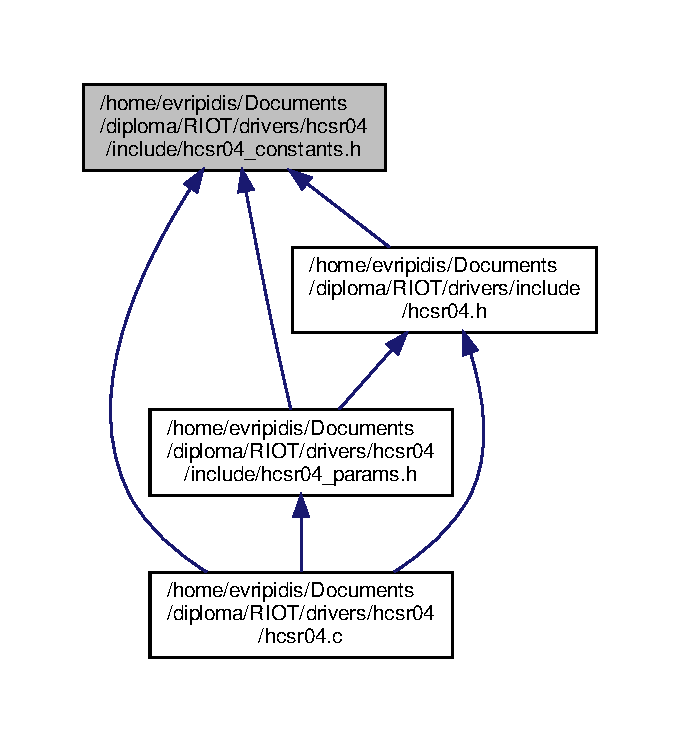
\includegraphics[width=327pt]{hcsr04__constants_8h__dep__incl}
\end{center}
\end{figure}
\subsection*{Macros}
\begin{Indent}\textbf{ H\+C-\/\+S\+R04 connection error value}\par
\begin{DoxyCompactItemize}
\item 
\mbox{\Hypertarget{hcsr04__constants_8h_a8152d1c4c747a366634d89a324bc7709}\label{hcsr04__constants_8h_a8152d1c4c747a366634d89a324bc7709}} 
\#define \hyperlink{hcsr04__constants_8h_a8152d1c4c747a366634d89a324bc7709}{E\+C\+ON}~(2\+U)
\begin{DoxyCompactList}\small\item\em Integer representing the error code. \end{DoxyCompactList}\end{DoxyCompactItemize}
\end{Indent}
\begin{Indent}\textbf{ H\+C-\/\+S\+R04 trigger duration}\par
\begin{DoxyCompactItemize}
\item 
\mbox{\Hypertarget{hcsr04__constants_8h_ade7e0a46b30c164eed780ea109c126ea}\label{hcsr04__constants_8h_ade7e0a46b30c164eed780ea109c126ea}} 
\#define \hyperlink{hcsr04__constants_8h_ade7e0a46b30c164eed780ea109c126ea}{T\+R\+I\+G\+G\+E\+R\+\_\+\+T\+I\+ME}~(10\+U)
\begin{DoxyCompactList}\small\item\em Duration time in us. \end{DoxyCompactList}\end{DoxyCompactItemize}
\end{Indent}
\begin{Indent}\textbf{ Distance limit parameters for H\+C\+S\+R04 ultrasonic sensor}\par
\begin{DoxyCompactItemize}
\item 
\mbox{\Hypertarget{hcsr04__constants_8h_a29227e726bd9572b55d4b92b7602c0ed}\label{hcsr04__constants_8h_a29227e726bd9572b55d4b92b7602c0ed}} 
\#define \hyperlink{hcsr04__constants_8h_a29227e726bd9572b55d4b92b7602c0ed}{H\+C\+S\+R04\+\_\+\+M\+I\+N\+\_\+\+D\+I\+S\+T\+A\+N\+C\+E\+\_\+\+MM}~(30\+U)
\begin{DoxyCompactList}\small\item\em Min distance possible in mm. \end{DoxyCompactList}\item 
\mbox{\Hypertarget{hcsr04__constants_8h_a0c6e7ee1cc90105baac932c3c8b16a9e}\label{hcsr04__constants_8h_a0c6e7ee1cc90105baac932c3c8b16a9e}} 
\#define \hyperlink{hcsr04__constants_8h_a0c6e7ee1cc90105baac932c3c8b16a9e}{H\+C\+S\+R04\+\_\+\+M\+A\+X\+\_\+\+D\+I\+S\+T\+A\+N\+C\+E\+\_\+\+MM}~(4000\+U)
\begin{DoxyCompactList}\small\item\em Max distance possible in mm. \end{DoxyCompactList}\end{DoxyCompactItemize}
\end{Indent}
\begin{Indent}\textbf{ Reference temperature}\par
\begin{DoxyCompactItemize}
\item 
\mbox{\Hypertarget{hcsr04__constants_8h_a4eab5906642820d9ba6e57a2b16bafa7}\label{hcsr04__constants_8h_a4eab5906642820d9ba6e57a2b16bafa7}} 
\#define \hyperlink{hcsr04__constants_8h_a4eab5906642820d9ba6e57a2b16bafa7}{R\+E\+F\+\_\+\+T\+E\+M\+P\+E\+R\+A\+T\+U\+RE}~(273.\+15\+F)
\begin{DoxyCompactList}\small\item\em Temperature in m Kelvin. \end{DoxyCompactList}\end{DoxyCompactItemize}
\end{Indent}
\begin{Indent}\textbf{ Speed of sound at the ref temperature for dry air}\par
\begin{DoxyCompactItemize}
\item 
\mbox{\Hypertarget{hcsr04__constants_8h_aa6b74c1a92a788d74ef3cb8e741ac757}\label{hcsr04__constants_8h_aa6b74c1a92a788d74ef3cb8e741ac757}} 
\#define \hyperlink{hcsr04__constants_8h_aa6b74c1a92a788d74ef3cb8e741ac757}{R\+E\+F\+\_\+\+S\+P\+E\+E\+D\+\_\+\+S\+O\+U\+ND}~(331.\+30\+F)
\begin{DoxyCompactList}\small\item\em Speed of sound in m/ms. \end{DoxyCompactList}\end{DoxyCompactItemize}
\end{Indent}
\begin{Indent}\textbf{ Temperature coefficient}\par
\begin{DoxyCompactItemize}
\item 
\mbox{\Hypertarget{hcsr04__constants_8h_a9e315b301a687e2440cdf4050cfdceb7}\label{hcsr04__constants_8h_a9e315b301a687e2440cdf4050cfdceb7}} 
\#define \hyperlink{hcsr04__constants_8h_a9e315b301a687e2440cdf4050cfdceb7}{C\+O\+E\+F\+F\+I\+C\+I\+E\+NT}~(\hyperlink{hcsr04__constants_8h_aa6b74c1a92a788d74ef3cb8e741ac757}{R\+E\+F\+\_\+\+S\+P\+E\+E\+D\+\_\+\+S\+O\+U\+ND} / sqrt(\hyperlink{hcsr04__constants_8h_a4eab5906642820d9ba6e57a2b16bafa7}{R\+E\+F\+\_\+\+T\+E\+M\+P\+E\+R\+A\+T\+U\+RE}))
\begin{DoxyCompactList}\small\item\em Converts data to appropriate form. \end{DoxyCompactList}\end{DoxyCompactItemize}
\end{Indent}


\subsection{Detailed Description}
Internal addresses, registers and constants. 

\begin{DoxyAuthor}{Author}
Evripidis Chondromatidis \href{mailto:eurichon1996@gmail.com}{\tt eurichon1996@gmail.\+com} 
\end{DoxyAuthor}

\hypertarget{hcsr04__params_8h}{}\section{/home/evripidis/\+Documents/diploma/\+R\+I\+O\+T/drivers/hcsr04/include/hcsr04\+\_\+params.h File Reference}
\label{hcsr04__params_8h}\index{/home/evripidis/\+Documents/diploma/\+R\+I\+O\+T/drivers/hcsr04/include/hcsr04\+\_\+params.\+h@{/home/evripidis/\+Documents/diploma/\+R\+I\+O\+T/drivers/hcsr04/include/hcsr04\+\_\+params.\+h}}


Default configuration.  


{\ttfamily \#include \char`\"{}board.\+h\char`\"{}}\newline
{\ttfamily \#include \char`\"{}hcsr04.\+h\char`\"{}}\newline
{\ttfamily \#include \char`\"{}hcsr04\+\_\+constants.\+h\char`\"{}}\newline
Include dependency graph for hcsr04\+\_\+params.\+h\+:\nopagebreak
\begin{figure}[H]
\begin{center}
\leavevmode
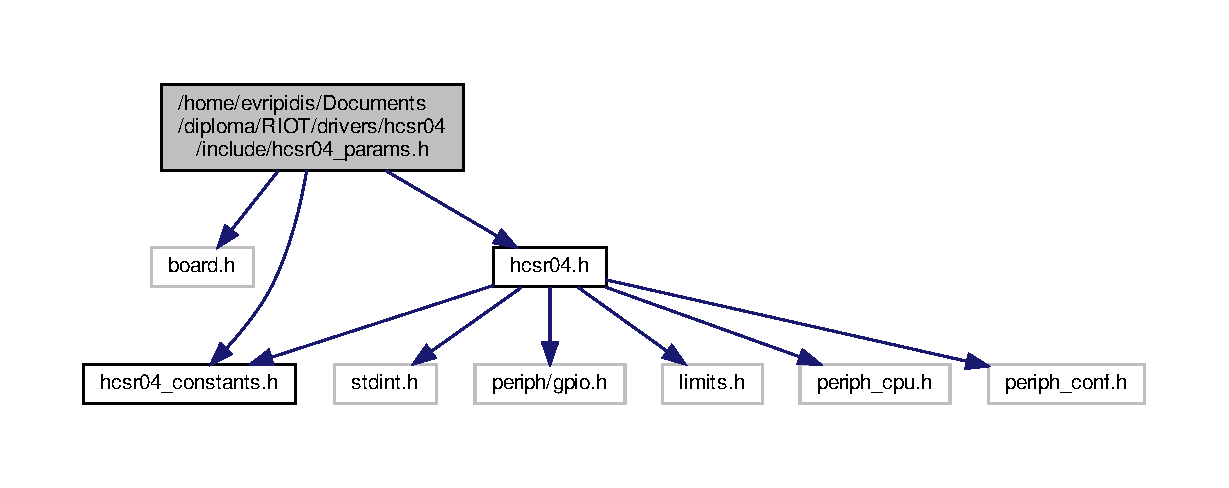
\includegraphics[width=350pt]{hcsr04__params_8h__incl}
\end{center}
\end{figure}
This graph shows which files directly or indirectly include this file\+:\nopagebreak
\begin{figure}[H]
\begin{center}
\leavevmode
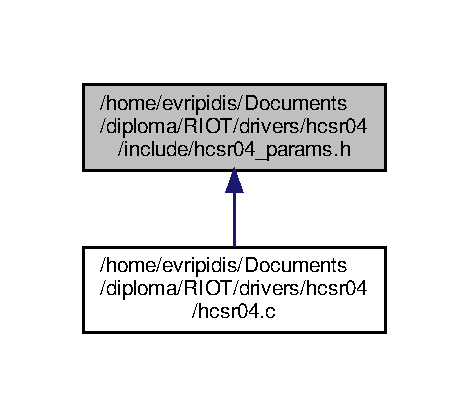
\includegraphics[width=225pt]{hcsr04__params_8h__dep__incl}
\end{center}
\end{figure}
\subsection*{Macros}
\begin{Indent}\textbf{ Default configuration parameters for H\+C-\/\+S\+R04 sensor}\par
\begin{DoxyCompactItemize}
\item 
\mbox{\Hypertarget{hcsr04__params_8h_ae32740e3781e1422c98eb463f0b306fe}\label{hcsr04__params_8h_ae32740e3781e1422c98eb463f0b306fe}} 
\#define {\bfseries A\+I\+R\+\_\+\+T\+E\+M\+P\+E\+R\+A\+T\+U\+RE}~(24000\+U)
\item 
\mbox{\Hypertarget{hcsr04__params_8h_a528ed4bcf450db7b92e45fd2c69706ad}\label{hcsr04__params_8h_a528ed4bcf450db7b92e45fd2c69706ad}} 
\#define {\bfseries H\+C\+S\+R04\+\_\+\+T\+R\+I\+G\+G\+E\+R\+\_\+\+P\+IN}~(G\+P\+I\+O\+\_\+\+P\+IN(0,2))
\item 
\mbox{\Hypertarget{hcsr04__params_8h_a5cd0a01008b3aec2301a56bc1ad7f231}\label{hcsr04__params_8h_a5cd0a01008b3aec2301a56bc1ad7f231}} 
\#define {\bfseries H\+C\+S\+R04\+\_\+\+E\+C\+H\+O\+\_\+\+P\+IN}~(G\+P\+I\+O\+\_\+\+P\+IN(0,4))
\item 
\#define \hyperlink{hcsr04__params_8h_a14070f879ab23d008c11418c63358ac2}{H\+C\+S\+R04\+\_\+\+P\+A\+R\+A\+MS}
\begin{DoxyCompactList}\small\item\em H\+C-\/\+S\+R04 default initialization parameters. \end{DoxyCompactList}\end{DoxyCompactItemize}
\end{Indent}


\subsection{Detailed Description}
Default configuration. 

\begin{DoxyAuthor}{Author}
Evripidis Chondromatidis \href{mailto:eurichon1996@gmail.com}{\tt eurichon1996@gmail.\+com} 
\end{DoxyAuthor}


\subsection{Macro Definition Documentation}
\mbox{\Hypertarget{hcsr04__params_8h_a14070f879ab23d008c11418c63358ac2}\label{hcsr04__params_8h_a14070f879ab23d008c11418c63358ac2}} 
\index{hcsr04\+\_\+params.\+h@{hcsr04\+\_\+params.\+h}!H\+C\+S\+R04\+\_\+\+P\+A\+R\+A\+MS@{H\+C\+S\+R04\+\_\+\+P\+A\+R\+A\+MS}}
\index{H\+C\+S\+R04\+\_\+\+P\+A\+R\+A\+MS@{H\+C\+S\+R04\+\_\+\+P\+A\+R\+A\+MS}!hcsr04\+\_\+params.\+h@{hcsr04\+\_\+params.\+h}}
\subsubsection{\texorpdfstring{H\+C\+S\+R04\+\_\+\+P\+A\+R\+A\+MS}{HCSR04\_PARAMS}}
{\footnotesize\ttfamily \#define H\+C\+S\+R04\+\_\+\+P\+A\+R\+A\+MS}

{\bfseries Value\+:}
\begin{DoxyCode}
\{ \(\backslash\)
                                                .temperature = AIR\_TEMPERATURE,  \(\backslash\)
                                                .trigger\_pin = HCSR04\_TRIGGER\_PIN,  \(\backslash\)
                                                .echo\_pin = HCSR04\_ECHO\_PIN,  \(\backslash\)
                                            \}
\end{DoxyCode}


H\+C-\/\+S\+R04 default initialization parameters. 


\hypertarget{hcsr04_8h}{}\section{/home/evripidis/\+Documents/diploma/\+R\+I\+O\+T/drivers/include/hcsr04.h File Reference}
\label{hcsr04_8h}\index{/home/evripidis/\+Documents/diploma/\+R\+I\+O\+T/drivers/include/hcsr04.\+h@{/home/evripidis/\+Documents/diploma/\+R\+I\+O\+T/drivers/include/hcsr04.\+h}}
{\ttfamily \#include $<$stdint.\+h$>$}\newline
{\ttfamily \#include \char`\"{}hcsr04\+\_\+constants.\+h\char`\"{}}\newline
{\ttfamily \#include \char`\"{}periph/gpio.\+h\char`\"{}}\newline
Include dependency graph for hcsr04.\+h\+:\nopagebreak
\begin{figure}[H]
\begin{center}
\leavevmode
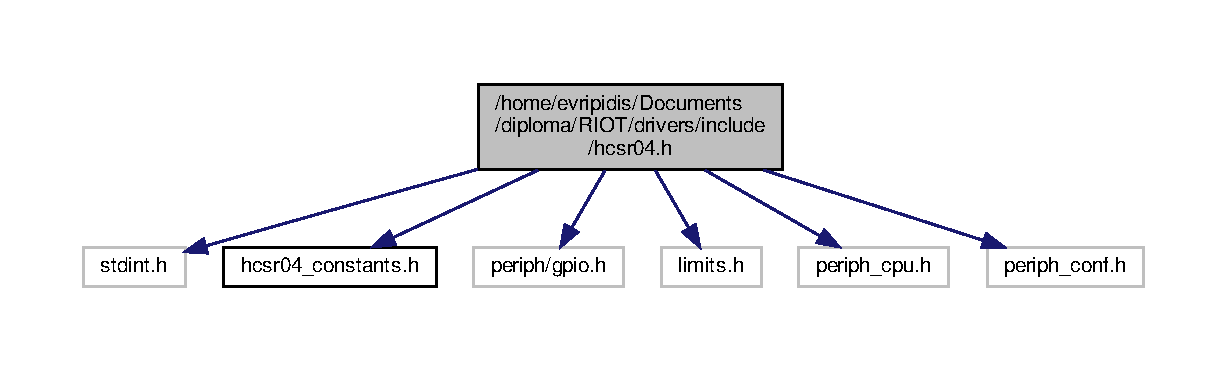
\includegraphics[width=350pt]{hcsr04_8h__incl}
\end{center}
\end{figure}
This graph shows which files directly or indirectly include this file\+:\nopagebreak
\begin{figure}[H]
\begin{center}
\leavevmode
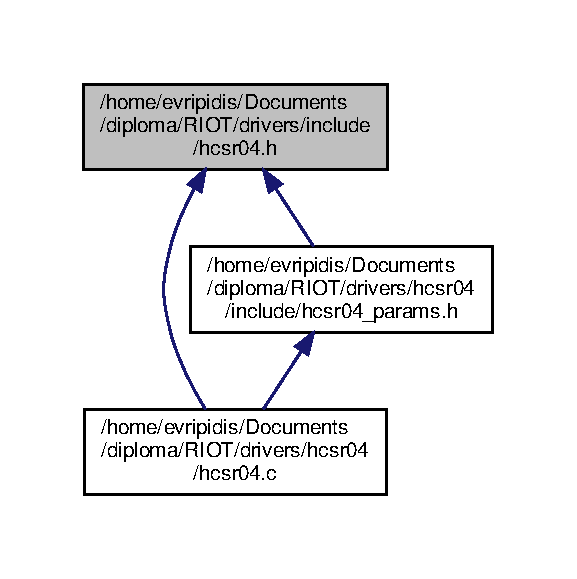
\includegraphics[width=277pt]{hcsr04_8h__dep__incl}
\end{center}
\end{figure}
\subsection*{Classes}
\begin{DoxyCompactItemize}
\item 
struct \hyperlink{structhcsr04__params__t}{hcsr04\+\_\+params\+\_\+t}
\begin{DoxyCompactList}\small\item\em Device initialization parameters for hcsr04 sensor. \end{DoxyCompactList}\item 
struct \hyperlink{structhcsr04__t}{hcsr04\+\_\+t}
\begin{DoxyCompactList}\small\item\em Device descriptor of a H\+C-\/\+S\+R04 sensor. \end{DoxyCompactList}\end{DoxyCompactItemize}
\subsection*{Functions}
\begin{DoxyCompactItemize}
\item 
int \hyperlink{group__drivers__hcsr04_gabcca3ead68bf012ae42e185e070cb764}{hcsr04\+\_\+init} (\hyperlink{structhcsr04__t}{hcsr04\+\_\+t} $\ast$dev, const \hyperlink{structhcsr04__params__t}{hcsr04\+\_\+params\+\_\+t} $\ast$params)
\begin{DoxyCompactList}\small\item\em Initialize an H\+C-\/\+S\+R04 sensor. \end{DoxyCompactList}\item 
void \hyperlink{group__drivers__hcsr04_gabbfe6e650342e8cc67cf9c9e81b29335}{hcsr04\+\_\+trigger} (\hyperlink{structhcsr04__t}{hcsr04\+\_\+t} $\ast$dev)
\begin{DoxyCompactList}\small\item\em Starts a measurement by triggering the H\+C-\/\+S\+R04 device. \end{DoxyCompactList}\item 
uint16\+\_\+t \hyperlink{group__drivers__hcsr04_ga449b9d4dc30d3d87d9ee4d8936fb592d}{hcsr04\+\_\+read} (\hyperlink{structhcsr04__t}{hcsr04\+\_\+t} $\ast$dev)
\begin{DoxyCompactList}\small\item\em Gets the last measurement reading. \end{DoxyCompactList}\item 
uint16\+\_\+t \hyperlink{group__drivers__hcsr04_ga3b2547facab2613e3113c2fd5d2bd6a8}{hcsr04\+\_\+temp\+\_\+to\+\_\+sound\+\_\+speed} (uint16\+\_\+t temp)
\begin{DoxyCompactList}\small\item\em Function that calculates the speed of sound. \end{DoxyCompactList}\item 
void \hyperlink{group__drivers__hcsr04_gad5a6694b723bb25fc48e7a8750b8a77a}{hcsr04\+\_\+set\+\_\+temp} (\hyperlink{structhcsr04__t}{hcsr04\+\_\+t} $\ast$dev, uint16\+\_\+t new\+\_\+temp)
\begin{DoxyCompactList}\small\item\em Function that sets the temperature. \end{DoxyCompactList}\item 
uint16\+\_\+t \hyperlink{group__drivers__hcsr04_gabef54fa09a72a7aa863aaa03b662125b}{hcsr04\+\_\+get\+\_\+distance} (\hyperlink{structhcsr04__t}{hcsr04\+\_\+t} $\ast$dev)
\begin{DoxyCompactList}\small\item\em Function that measures the current distance. \end{DoxyCompactList}\end{DoxyCompactItemize}


\subsection{Detailed Description}
\begin{DoxyAuthor}{Author}
Evripidis Chondromatidis \href{mailto:eurichon1996@gmail.com}{\tt eurichon1996@gmail.\+com} 
\end{DoxyAuthor}

%--- End generated contents ---

% Index
\backmatter
\newpage
\phantomsection
\clearemptydoublepage
\addcontentsline{toc}{chapter}{Index}
\printindex

\end{document}
